\section{Berechnung des Lenkwinkels}

\begin{figure}[H] % [htb]
  \centering
  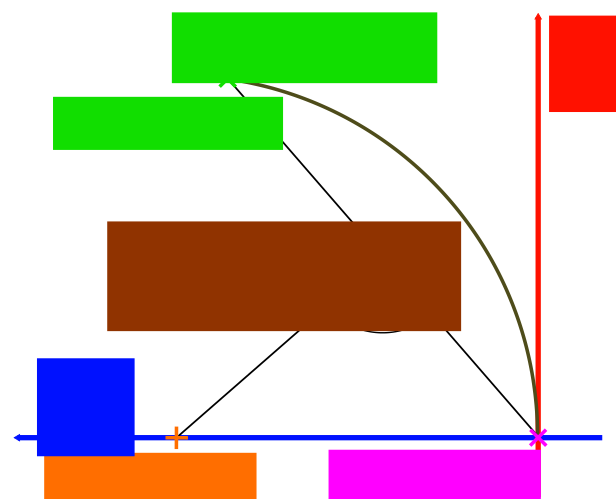
\includegraphics[width=0.8\textwidth]{regelung_lenkwinkel_radius.pdf}
  \caption{Veranschaulichung zur Bestimmung des Kreisradius aus dem gegebenen Zielpunkt in Roboterkoordinaten}
  \label{fig:regelung_lenkwinkel_radius}
\end{figure}

\begin{eqnarray}
\text{Gerade 1:  } y & = & m_G \cdot x + n_G 	\\
\text{Gerade 2:  } y & = & m_H \cdot x + n_H
\end{eqnarray}

\begin{eqnarray}
 m_G = \frac{\Delta y}{\Delta x} & = & \frac{y_G}{x_G} 	\\
 m_H = \frac{\Delta y}{\Delta x} & = & \frac{x_G}{-y_G}
\end{eqnarray}

\begin{eqnarray}
x_H & = & 0.5 \cdot x_G 	\\
y_H & = & 0.5 \cdot y_G
\end{eqnarray}

\begin{equation}
r = n_H = y_H - m_H \cdot x_H = 0.5 \cdot (y_G + \frac{{x_G}^2}{y_G} )
\end{equation}